%%% Global variables
\newcommand{\weekNum}{1}




\documentclass[12pt]{article}
\usepackage[english]{babel}
\usepackage{natbib}
\usepackage{url}
\usepackage[utf8x]{inputenc}
\usepackage{amsmath}
\usepackage{graphicx}

\graphicspath{{images/}}
\usepackage{parskip}
\usepackage{fancyhdr}
\usepackage{vmargin}
\usepackage{tikz}
\usetikzlibrary{positioning}
\setmarginsrb{3 cm}{2.5 cm}{3 cm}{2.5 cm}{1 cm}{1.5 cm}{1 cm}{1.5 cm}


							


\makeatletter
\let\thetitle\@title

\let\thedate\@date
\makeatother

\pagestyle{fancy}
\fancyhf{}
\rhead{\theauthor}
\lhead{\thetitle}
\cfoot{\thepage}


\begin{document}

%%%%%%%%%%%%%%%%%%%%%%%%%%%%%%%%%%%%%%%%%%%%%%%%%%%%%%%%%%%%%%%%%%%%%%%%%%%%%%%%%%%%%%%%%

\begin{titlepage}
	\centering
    \vspace*{0.5 cm}
    
\includegraphics[scale = 1.5]{METU_Logo.jpg}\\[1.0 cm]	% University Logo
    \textsc{\Large MIDDLE EAST TECHNICAL} \\[0.2 cm]
    \textsc{\Large UNIVERSITY} \\ [2.0 cm]
    \textsc{\large ELECTRICAL \& ELECTRONICS ENGINEERING} \\[0.2 cm]
    \textsc{\large Weekly Report \weekNum}\\[0.2 cm]
	\textsc{\large EE 493}\\[0.5 cm]				% Course Code
	\textsc{\large Cat Feeding Project}\\[0.2 cm]
	\rule{\linewidth}{0.2 mm} \\[0.4 cm]
	{ \huge \bfseries \thetitle}
	
	\begin{minipage}{0.4\textwidth}
		
			\begin{flushright} 
			\emph{STUDENT ID :} \\
			2166387\linebreak
			
			% Your Student Number
		\end{flushright}
	\end{minipage}\\[2 cm]
	

 
	\vfill
	
\end{titlepage}

%%%%%%%%%%%%%%%%%%%%%%%%%%%%%%%%%%%%%%%%%%%%%%%%%%%%%%%%%%%%%%%%%%%%%%%%%%%%%%%%%%%%%%%%%

\tableofcontents
\pagebreak

%%%%%%%%%%%%%%%%%%%%%%%%%%%%%%%%%%%%%%%%%%%%%%%%%%%%%%%%%%%%%%%%%%%%%%%%%%%%%%%%%%%%%%%%%

\section{INTRODUCTION}
Cat feeding project report \weekNum is presented in this report. This week we have done a lot of works in various aspects of the project. Therefore, it is best to present the results in sections mechanic design, electronic component selection, base software development, computer vision which are given as sections \ref{sec:mechanic}, \ref{sec:electronic}, \ref{sec:software} and \ref{sec:vision} respectively. The tasks for the next week is given in section \ref{sec:tasks}.

...TODO - overall sistem aciklanabilir

We shared the work according to our abilities and professions. We end up with the following work structure:


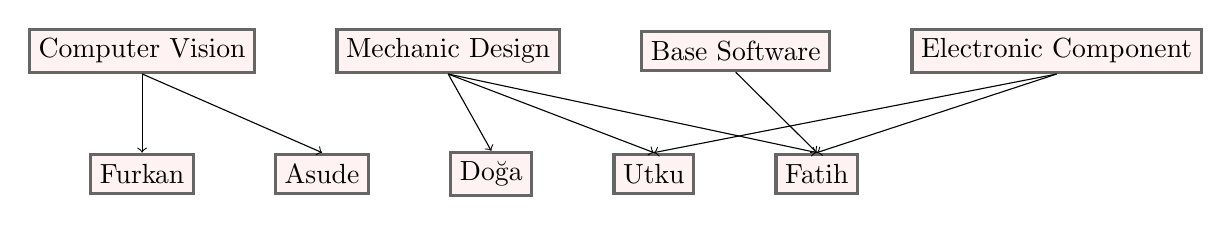
\begin{tikzpicture}[
roundnode/.style={circle, draw=green!60, fill=green!5, very thick, minimum size=7mm},
squarednode/.style={rectangle, draw=black!60, fill=red!5, very thick, minimum size=5mm},
]
% Nodes here..
\node[squarednode] (vis) {Computer Vision};
\node[squarednode] (mec) [right=of vis] {Mechanic Design};
\node[squarednode] (soft) [right=of mec] {Base Software};
\node[squarednode] (ele) [right=of soft] {Electronic Component};
\node[squarednode] (furkan) [below=of vis] {Furkan};
\node[squarednode] (asude) [right=of furkan] {Asude};
\node[squarednode] (doga) [right=of asude] {Doğa};
\node[squarednode] (utku) [right=of doga] {Utku};
\node[squarednode] (fatih) [right=of utku] {Fatih};

% Draw lines..
\draw[->] (mec.south) -- (fatih.north);
\draw[->] (mec.south) -- (utku.north);
\draw[->] (mec.south) -- (doga.north);

\draw[->] (vis.south) -- (furkan.north);
\draw[->] (vis.south) -- (asude.north);

\draw[->] (ele.south) -- (fatih.north);
\draw[->] (ele.south) -- (utku.north);

\draw[->] (soft.south) -- (fatih.north);

\end{tikzpicture}

\section{Mechanic Design} \label{sec:mechanic}
This week the overall mechanical design was discussed. By observing the similar systems, a rude concept of the design was made.  Mechanical design part was divided into two categories: Inner design and Outer design.
Inner design might be problematic since it includes the food and water tank systems. In order to control the amount of the cat food which will flow through food container, the gate should be designed and this gate should effectively cut the food flow. We have think about some gates like using magnets for holding the door or using a system like spinning wheel. However in first case the power of the magnet might not enough for holding the door therefore we have to make some editions in order to make it work. Moreover due to the magnets magnetic field other devices might be suffer. In the second case the spinning wheel might also cause some problems like, it might not rotate due to the friction between food and bucket. Moreover in order to implement it one has to use powerful motor and due to the size of the spinning wheel the overall systems will be huge, which is not desirable for aesthetic and economic reasons. On the other hand we came up with an idea that we can use a systems like ordinary salts have. One can see this on figure \ref{fig:tuzluk}

\begin{figure}
    \centering
    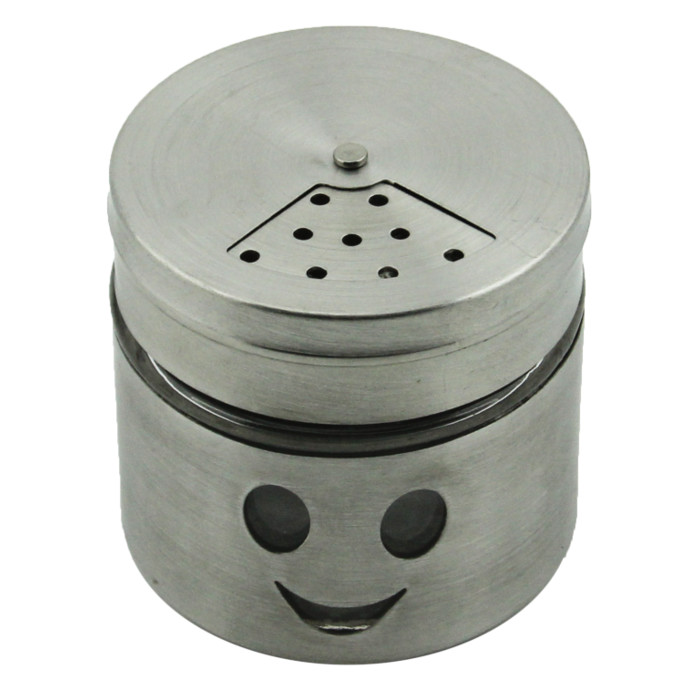
\includegraphics[width=.5\linewidth]{Tuzluk.jpg}
    \caption{Salt Cup}
    \label{fig:tuzluk}
\end{figure}

This systems is applicable since one can control the flow of the food by rotating the cover of the salt cup. When two open sides are matched food flows however when one open side matches with a closed side of the cover food flow stops.
Outer design will be handled when the inner design is fixed since, the dimensions of it will be determined by the system which be implemented inside. 

...TODO
\pagebreak

\section{Electronic Component Selection}
\label{sec:electronic}
The main constraints of the hardware selection is the power consumption, communication capability, network performance and software support. TODO - genel bir arastirma yaptik iste sunu sunu kullanalim dedik falan filan
baglanti semasi gelebilir, cihazlarin resimleri gelebilir
...TODO
\pagebreak

\section{Base Software Development}
\label{sec:software}

Neural networks and feature descriptors are decided to be used for cat and dog classification. Since embedded electronic computers are not capable of doing mass works, it is concluded that a server is going to be used. As a result, it became a must to transfer data from the embedded system to the powerful computer. The transfer process is done over network socket with TCP protocol.

To transfer data properly and make the whole system consistent, a schema of software overview is designed. Figure \ref{fig:overallView} shows the rough schema that how the network is constructed and related to the other components of the project such as computer vision, database, starting cat feeder.

\begin{figure}
    \centering
    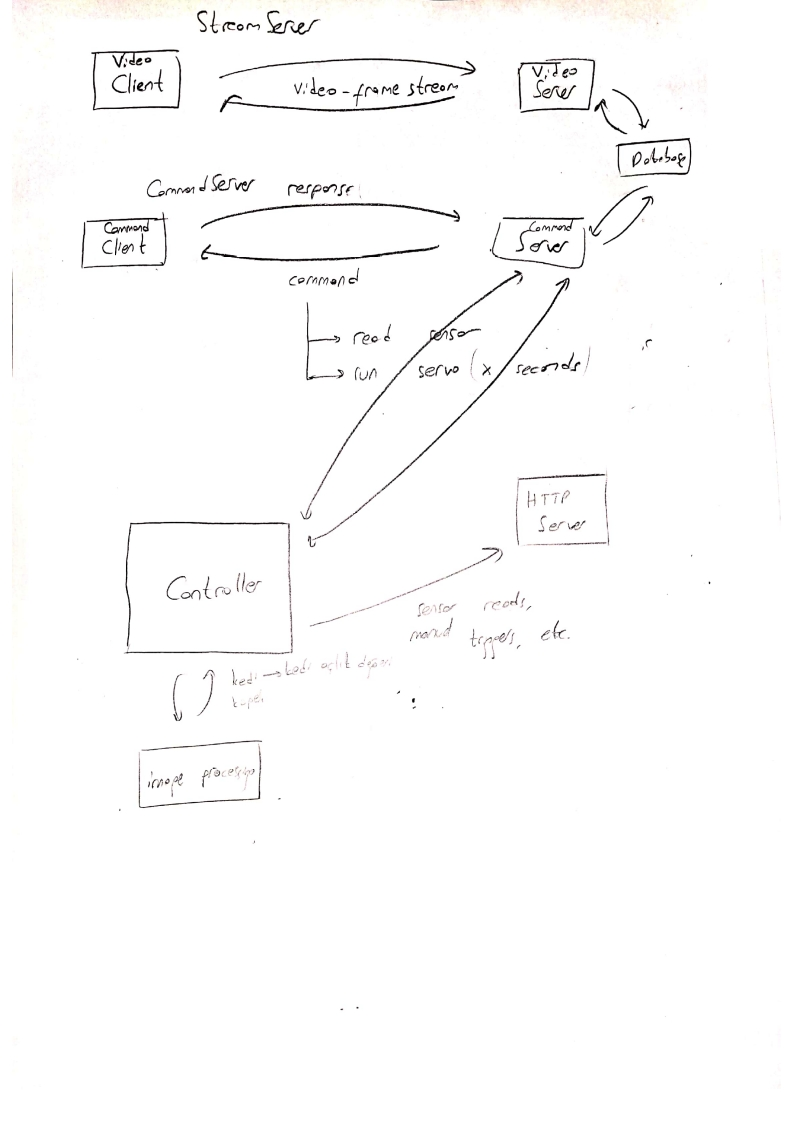
\includegraphics[width=0.98\linewidth]{SchemaSharpened.jpg}
    \caption{Overall System Schema}
    \label{fig:overallView}
\end{figure}

Native implementation of python of ServerSocket and Socket objects are used. This part of the work includes the data transfer, video streaming and frame transfer, command transfer and response. This week is mainly about transferring a single frame over network and abstract object structures for client-server and camera driver objects. More specifically, camera driver(CameraDriver.py) and server-client(ServerClient.py) source files are started and some basic functionalities are added. Note that currenly the source code is being developed under pi branch in GitHub which will then be rebased so that minimum congestion arises.

Parameter optimization for the data transfer is the another factor which affect the data transfer performance and stability of the transferred image. Using greater number of frames and low data buffer sizes, the image is transferred partially, or even the first segments are broken which caused the corrupted data. The system is still needed to be improved and integrated with the computer vision work group of the project.
\pagebreak

\section{Computer Vision}
\label{sec:vision}
...TODO
\pagebreak


\section{Next Week Tasks}
\label{sec:tasks}
...TODO
\pagebreak


\section{Conclusion}
\label{sec:conclusion}
...TODO

\newpage
\bibliographystyle{plain}
\bibliography{biblist}

\end{document}
